\documentclass[12pt]{article} % use larger type; default would be 10pt

\linespread{1.25}

\usepackage[margin=1in]{geometry}
\usepackage[english]{babel}
\usepackage[utf8x]{inputenc}
\usepackage{multirow}
\usepackage{multicol}
\usepackage{graphicx}
\usepackage{float}
\usepackage{tabu}
\usepackage{epstopdf}
\usepackage{rotating}
\usepackage{pdflscape}
\usepackage{setspace}
\usepackage[toc,page]{appendix}
\usepackage[round]{natbib}
\usepackage{booktabs}   % for nice tables
\usepackage{kpfonts}    % for nice fonts
\usepackage{microtype}
\usepackage[T1]{fontenc}
\usepackage{listings}   % for inserting code
\usepackage{paralist} % very flexible & customisable lists (eg. enumerate/itemize, etc.)
\usepackage{verbatim} % adds environment for commenting out blocks of text & for better verbatim
\usepackage{subcaption}
\usepackage{fancyhdr} % This should be set AFTER setting up the page geometry
\usepackage{caption}
\usepackage{float}
\usepackage{color}  
\usepackage[colorlinks=true]{hyperref}
\usepackage[colorinlistoftodos]{todonotes}
\usepackage{ragged2e}

% maths
\usepackage{mathtools}
\usepackage{amsthm}
\usepackage{amsmath}
\usepackage{amssymb}
\usepackage{bbm}
\usepackage{tikz}
\newcommand{\Mypm}{\mathbin{\tikz [x=1.4ex,y=1.4ex,line width=.1ex] \draw (0.0,0) -- (1.0,0) (0.5,0.08) -- (0.5,0.92) (0.0,0.5) -- (1.0,0.5);}}
\newcommand{\R}{\mathbb{R}} 
\renewcommand{\headrulewidth}{0pt} 
\lhead{}\chead{}\rhead{}
\lfoot{}\cfoot{\thepage}\rfoot{}

\DeclareMathOperator*{\argmax}{arg \, max}
\DeclareMathOperator*{\argmin}{arg \, min}
\DeclareMathOperator*{\var}{var}
\DeclareMathOperator*{\cov}{cov}

\theoremstyle{plain}
\newtheorem{definition}{Definition}
\newtheorem{proposition}{Proposition}
\newtheorem{lemma}{Lemma}
\newtheorem{corollary}{Corollary}
\newtheorem{remark}{Remark}

\theoremstyle{definition}
\newtheorem{assumption}{Assumption}
\newtheorem{dfn}{Definition}

\graphicspath{{figures/}}

\usepackage{cleveref} % for clever ref 
\usepackage{array}    % for better arrays (eg matrices) in maths
\usepackage{datetime2}
\usepackage{qtree}

\usepackage{hyperref}
\hypersetup{
	colorlinks   = true,
	citecolor    = blue,
	urlcolor 	 = blue,
	linkcolor    = black 
}

%%% SECTION TITLE APPEARANCE
\usepackage{sectsty}
\allsectionsfont{\sffamily\mdseries\upshape} % (See the fntguide.pdf for font help)
\usepackage[nottoc,notlof,notlot]{tocbibind} % Put the bibliography in the ToC
\usepackage[titles,subfigure]{tocloft} % Alter the style of the Table of Contents
\renewcommand{\cftsecfont}{\rmfamily\mdseries\upshape}
\renewcommand{\cftsecpagefont}{\rmfamily\mdseries\upshape} % No bold!

\author{ \textsc{Jonathan Créchet}\thanks{Department of Economics, University of Ottawa; jcrechet@uottawa.ca.} }

\title{Heterogeneity in labor mobility and unemployment flows across countries -- Figures}

\date{March 2023}

\begin{document}
	
	\maketitle
	
	\noindent \textbf{JEL: } E24, J60.
	
	\noindent \textbf{Keywords: } Unemployment, worker flows, search frictions, heterogeneity, labor-market institutions, firing costs.
	
	\newpage
		
	\begin{figure}[!h]
		\centering
		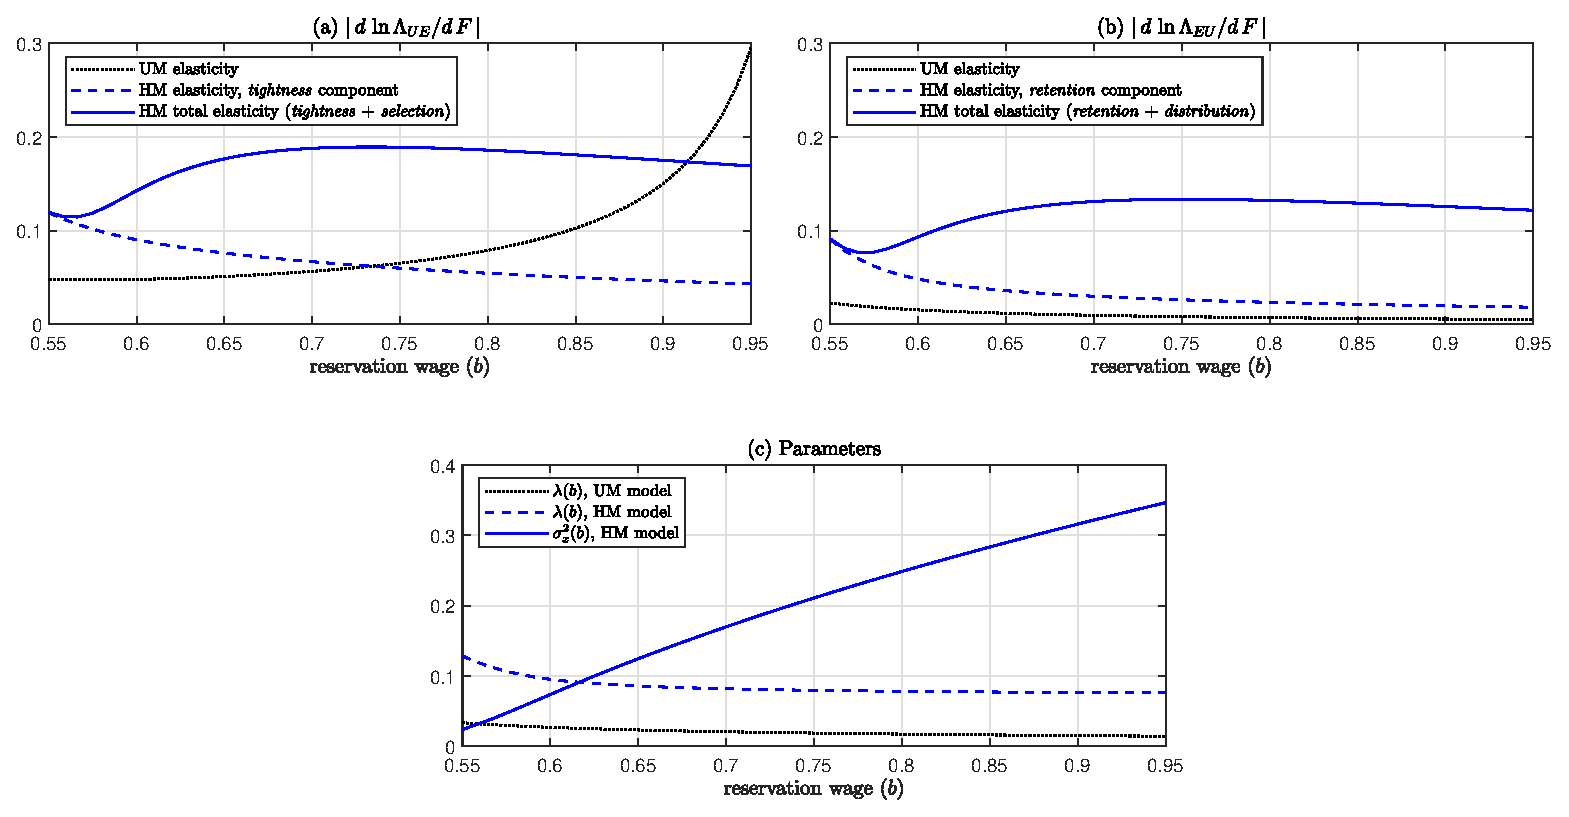
\includegraphics[width=6in]{Figures/Figure_1.eps}
		\caption{Semi-elasticities across values of the reservation wage in the calibrated models}
		    \caption*{
			\footnotesize \textit{Notes}: panel (a): semi-elasticity of the steady state unemployment-to-employment (UE) rate in the uniform-mobility (UM) and heterogeneous mobility (HM) models with respect to firing costs, for different values of non-work utility $b$ (and the associated values $\lambda(b)$, $\sigma_x(b)^2$, presented in panel(c)). Panel (b): semi-elasticity of the employment-to-unemployment (EU) rate. Panel (c): value of the stochastic shock $\lambda(b)$ and the variance of match quality $\sigma_x^2(b)$ required to match the calibration targets discussed in the main text. The UM elasticities are based on expressions \eqref{theory:UE:nohet} and \eqref{theory:EU:nohet}. The HM elasticities and the associated components are based on expressions \eqref{theory:dUE:het} and \eqref{theory:dEU:het}.}
		\label{fig:fig_1}
	\end{figure}

	\begin{figure}[!h]
	\begin{subfigure}{0.50\textwidth}
		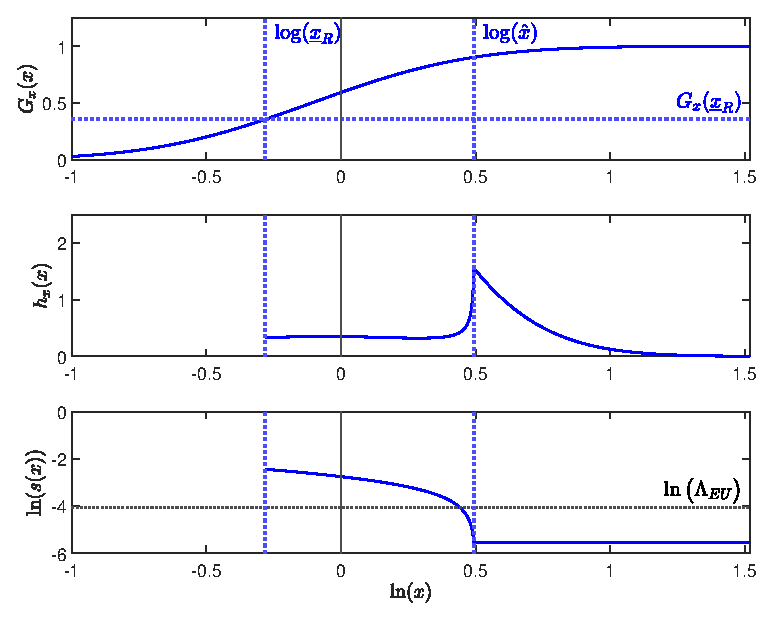
\includegraphics[width=1\linewidth]{Figure_2a.eps}
		\caption{Equilibrium with no firing costs}
	\end{subfigure}
	\begin{subfigure}{0.50\textwidth}
		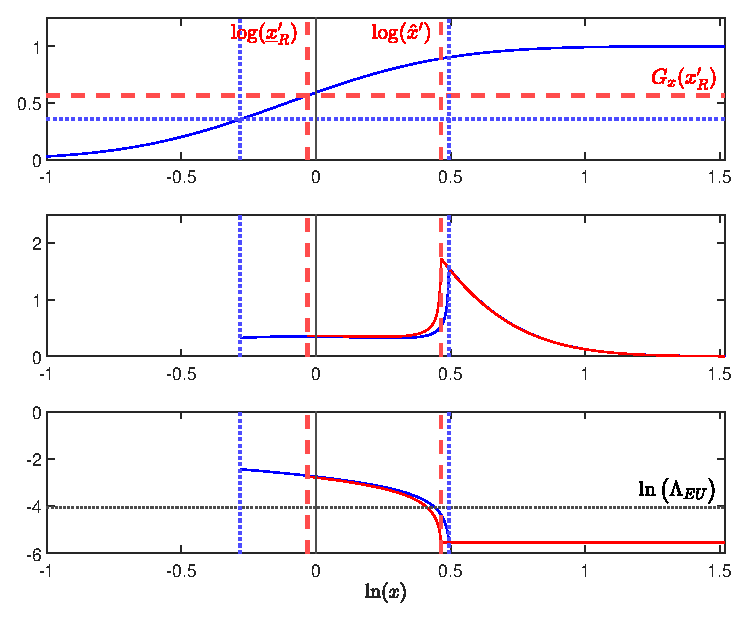
\includegraphics[width=1\linewidth]{Figure_2b.eps}
		\caption{Equilibrium with positive firing costs}
	\end{subfigure}
	\caption{Equilibrium effects of firing costs in the model with heterogeneous mobility.}
	\caption*{\footnotesize \textit{Notes}: illustration of equilibrium match-quality distributions and policy functions in the model with heterogeneity in permanent match quality for $F=0$ (panel (a)) and $F=3$ (panel (b)). Parameter values: $b = 0.75$; $\lambda = 0.084$; $\sigma_x^2 = 0.216$. All figures have the match quality in log terms in the horizontal axis and show vertical lines for (i) the hiring thresholds ($\underline{x}_R$ and $\underline{x}_R'$, with the prime subscript ($'$) referring to the equilibrium solution for $F=3$); (ii) the inaction cutoffs ($\hat{x}$ and $\hat{x}'$). Top panels: unconditional cumulative distribution $G_x$; middle: equilibrium probability distribution functions $h_x$ and $h_x'$; bottom: separation probabilities conditional on match quality, $s_x$ and $s_x'$, jointly with the targeted aggregate EU rate (equal to 1.73\%).}
	\label{fig:fig_2}
	\end{figure}

	\begin{figure}[!h]
	\begin{subfigure}{.5\textwidth}
		\centering		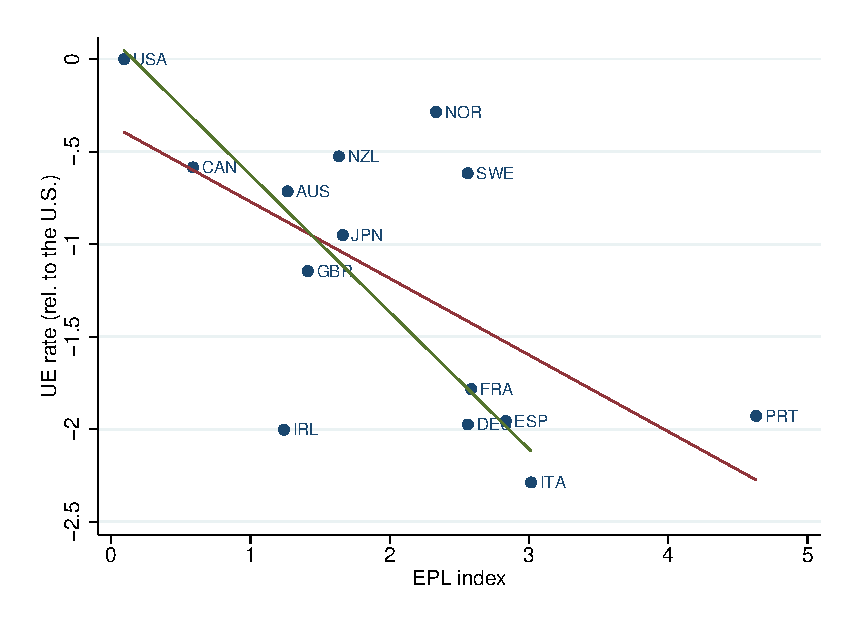
\includegraphics[width=1\linewidth]{Figure_3a.eps}
		\caption{UE monthly transition probability}
	\end{subfigure}
	\begin{subfigure}{.5\textwidth}
		\centering
		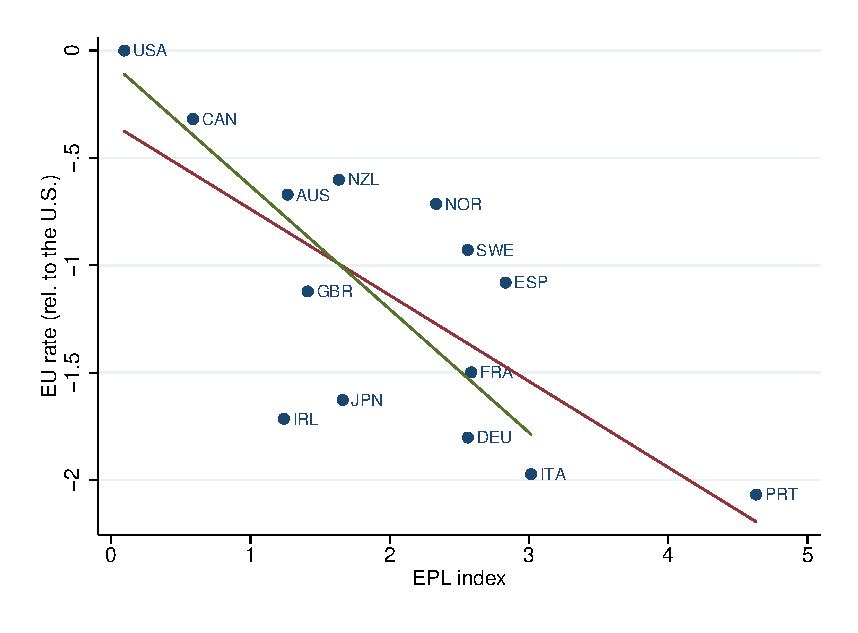
\includegraphics[width=1\linewidth]{Figure_3b.eps}
		\caption{EU monthly transition probability}
	\end{subfigure}
	\caption{OECD EPL index and unemployment flows across countries, 1990-2009.}
			\caption*{
		\footnotesize \textit{Notes}: unemployment-to-employment (UE) and employment-to-unemployment (EU) monthly transition probabilities and OECD Employment protection legislation (EPL) index values for select countries. The transition probabilities are computed using the monthly hazard rates by country estimated by \cite*{elsby_hobijn_sahin_2013_Restat}, averaged over the period 1990-2009. For each country, the average transition probabilities are reported in relative deviation from the U.S.\ averages. The OECD EPL index (individual dismissals, regular contracts--version 1) is obtained from OECD Statistics (\url{https://stats.oecd.org/}). The EPL index is averaged over the sample period. The green regression line excludes the less populated European countries (Ireland, Norway, Portugal, Sweden).}
	\label{fig:fig_3}
	\end{figure}
	
	\begin{figure}[!h]
		\centering
		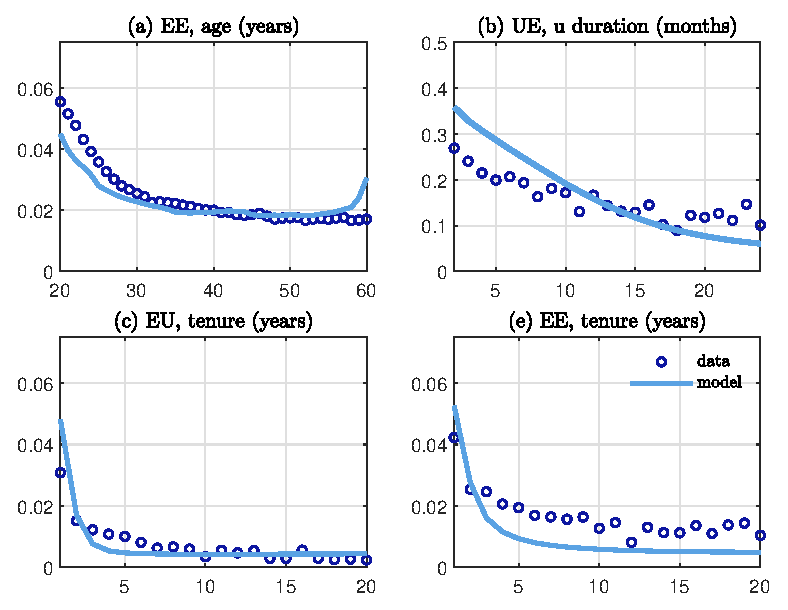
\includegraphics[width = 4.5in]{Figure_4.eps} 
		\caption{Model fit to \text{untargeted} empirical transition profiles.}
			\caption*{\footnotesize \textit{Notes}: untargeted empirical and model age, unemployment duration, and job-tenure monthly transition probabilities. Data source: IPUMPS CPS, 1995-2018.  Empirical profiles computed from worker-flow data constructed using Basic Monthly files and Job Tenure Supplements. See data appendix \ref{appendix:data}.}
		\label{fig:fig_5}
	\end{figure}

	\newpage
	
	\begin{figure}[!h]
		\centering
		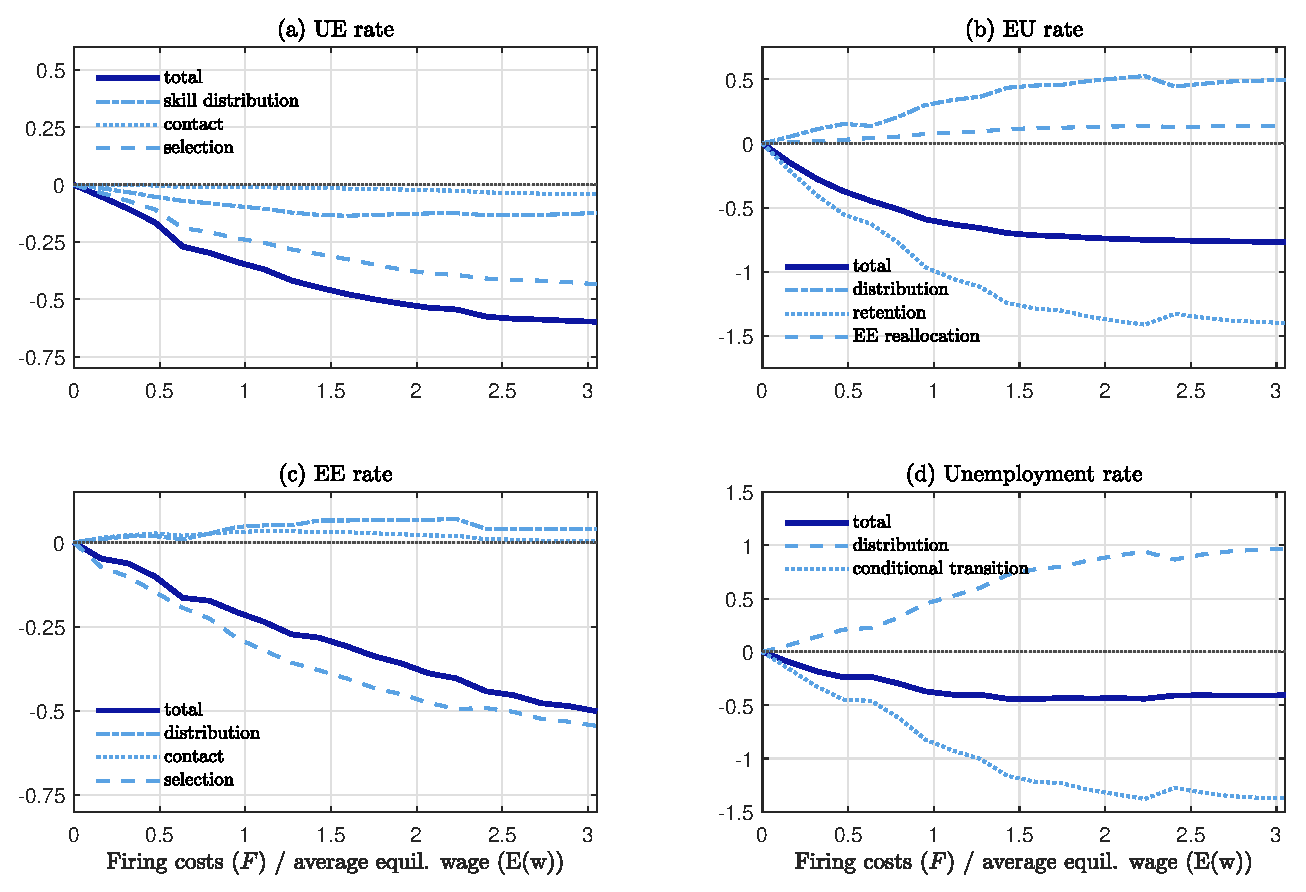
\includegraphics[width = 6.5in]{Figure_5.eps} 
		\caption{Decomposition of the effect of firing costs on steady-state equilibrium outcomes.}
		\label{fig:fig_6}
		\caption*{\footnotesize{\textit{Notes:} decomposition of quantitative model UE, EU, EE, unemployment statics percentage variations in response to changes in firing costs (expressed in average equilibrium wage equivalent. The decomposition is based on section 4.5. Each line represents the relative variation in a component. The ``contact'' UE component is the sum of the tightness and search UE components. The ``distribution'' and ``conditional-transition'' unemployment-rate components sum up components of the UE and EU elasticities.}}
	\end{figure}
	
	\begin{figure}[!h]
		\centering
		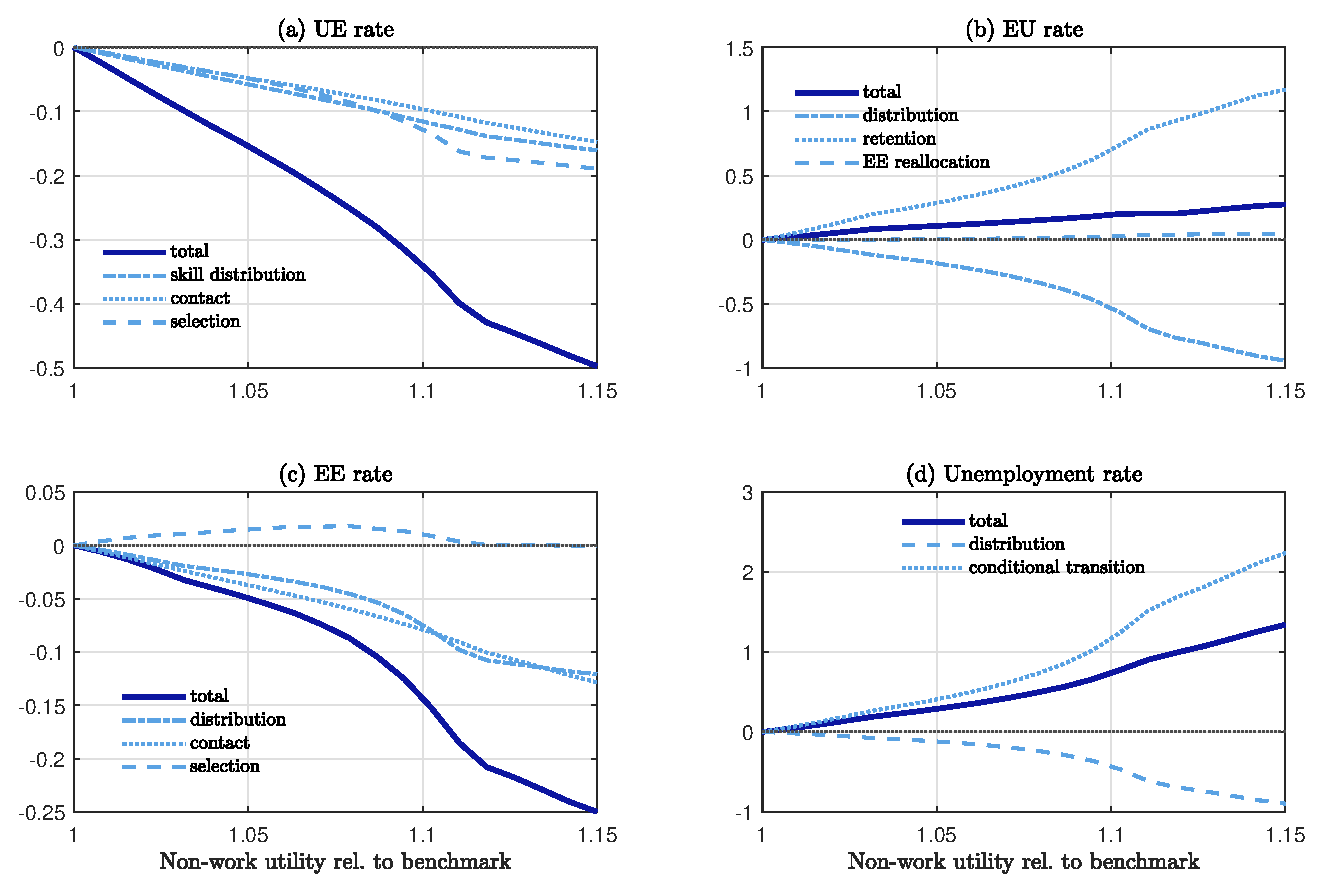
\includegraphics[width = 6.5in]{Figure_6.eps} 
		\caption{Decomposition of the effect of higher non-work utility on steady-state equilibrium outcomes}
		\label{fig:fig_7}
		\caption*{\footnotesize{\textit{Notes:} decomposition of quantitative model UE, EU, EE, unemployment statics percentage variations in response to changes in non-work utility $b$ relative to its benchmark counterpart value. The decomposition is based on section 4.5. Each line represents the relative variation in a component. The ``contact'' UE component is the sum of the tightness and search UE components. The``distribution'' and ``conditional-transition'' unemployment-rate components sum up components of the UE and EU elasticities.}}
	\end{figure}
	
	\begin{figure}[!h]
		\centering
		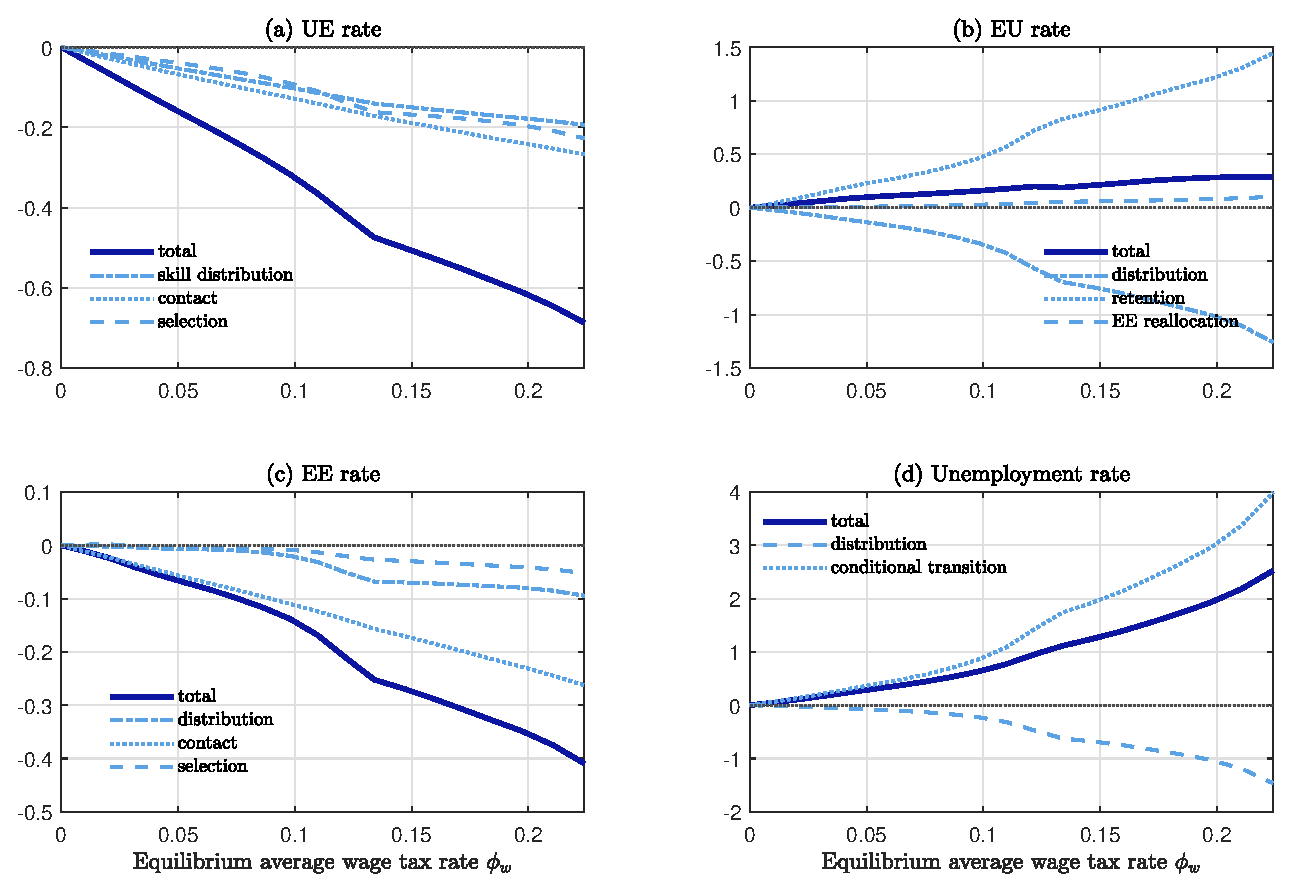
\includegraphics[width = 6.5in]{Figure_7.eps} 
		\caption{Decomposition of the effect of a higher proportional tax on wages on steady-state equilibrium outcomes}
		\label{fig:fig_8}
		\caption*{\footnotesize{\textit{Notes:} decomposition of quantitative model UE, EU, EE, unemployment statics percentage variations in response to changes in match-output average collected tax as a share of the average equilibrium wage (the parameter $\tau_P$). The decomposition is based on section 4.5. Each line represents the relative variation in a component. The ``contact'' UE component is the sum of the tightness and search UE components. The``distribution'' and ``conditional-transition'' unemployment-rate components sum up components of the UE and EU elasticities.}}
	\end{figure}
	
	\begin{figure}[!h]
		\centering
		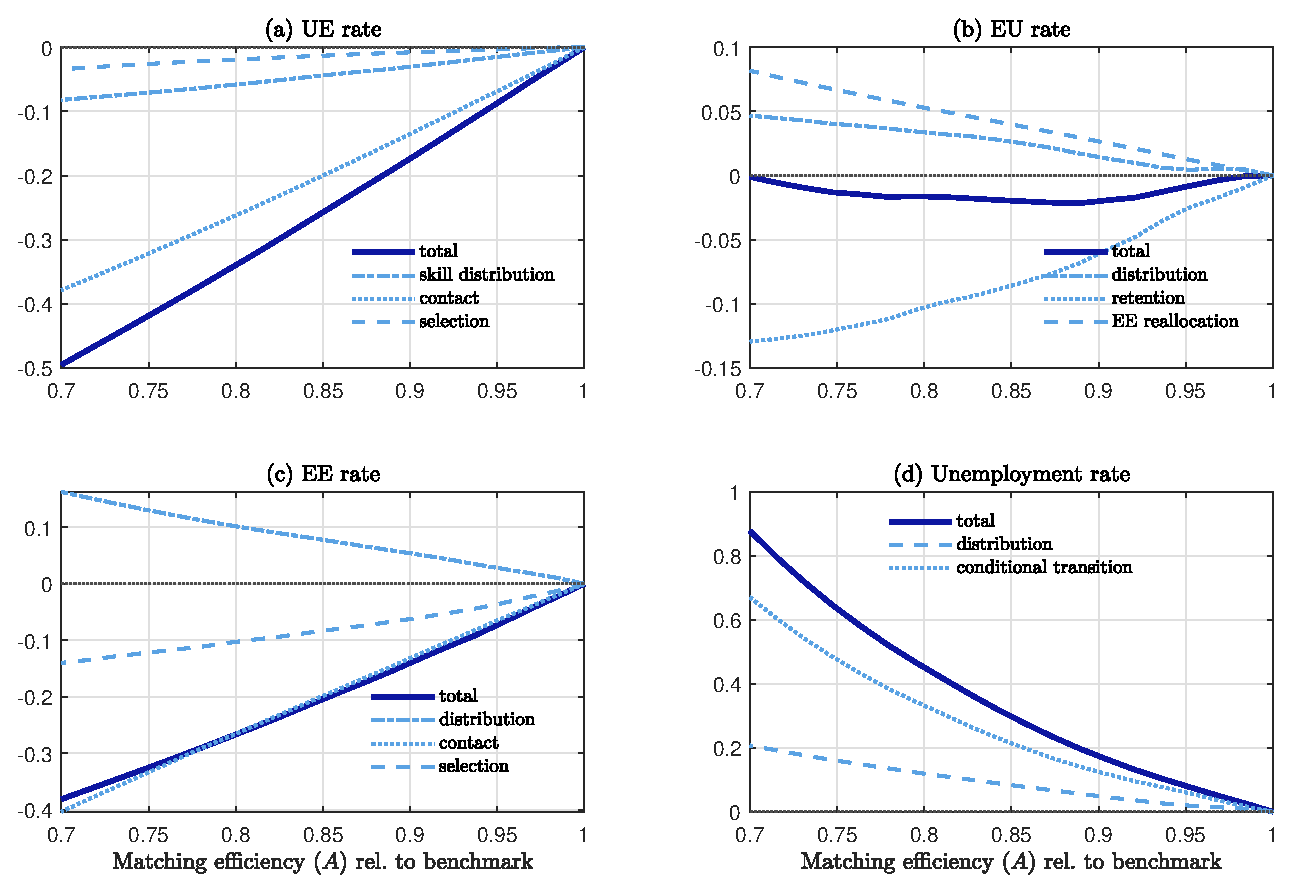
\includegraphics[width = 6.5in]{Figure_8.eps} 
		\caption{Decomposition of the effect of lower matching efficiency on steady-state equilibrium outcomes}
		\label{fig:fig_9}
		\caption*{\footnotesize{\textit{Notes:} decomposition of quantitative model UE, EU, EE, unemployment statics percentage variations in response to changes in matching efficiency $A$ relative to its benchmark counterpart value. The decomposition is based on section 4.5. Each line represents the relative variation in a component. The ``contact'' UE component is the sum of the tightness and search UE components. The``distribution'' and ``conditional-transition'' unemployment-rate components sum up components of the UE and EU elasticities.}}
	\end{figure}
	
\end{document}






